\documentclass[12pt,twoside, a4paper, twocolumn]{article}
\usepackage[utf8]{inputenc}
\usepackage[brazil]{babel}
\usepackage[margin = 0.5in]{geometry}
\usepackage{amsmath}
\usepackage{amsthm}
\usepackage{amssymb}
\usepackage{amsthm}
\usepackage{setspace}
\usepackage[americanvoltages,fulldiodes,siunitx]{circuitikz}
\usepackage{lipsum}
\usepackage{pgfplots}
\usepackage{ifthen}
\usepackage{adjustbox}
\usepackage[section]{placeins}
\usepackage{hyperref}
\usepackage{graphicx}
\usepackage{amsmath}
\usepackage{amsthm}
\usepackage{amssymb}
\usepackage{amsthm}
\usepackage{setspace}
\usepackage[americanvoltages,fulldiodes,siunitx]{circuitikz}
\usepackage{lipsum}
\usepackage{pgfplots}
\usepackage{ifthen}
\usepackage{adjustbox}
\usepackage[section]{placeins}
\usepackage{hyperref}
\usepackage{graphicx}
\usepackage{adjustbox}
\usepackage{indentfirst}
\usepackage{float}
\usepackage{pythonhighlight}


\pgfplotsset{compat=newest}
\graphicspath{ {./images/} }
%  #1 color - optional #2 x_0 #3 y_0 #4 x_f #5 y_f #6 name - optional  #7 true if adding lines to axis
\newcommand{\drawvector} [9] [color=cyan] {
\draw[line width=1.5pt,#1,-stealth](axis cs: #2, #3)--(axis cs: #4, #5) node[anchor=south west]{$#6$};
\ifthenelse{\equal{#7}{true}}{
\draw[line width=1pt,#1, dashed](axis cs: #4, #5)--(axis cs: #4, 0) node[anchor= north west]{$#8$};
\draw[line width=1pt,#1, dashed](axis cs: #4, #5)--(axis cs: 0, #5) node[anchor=south east]{$#9$};
}
{}
}
\newcommand\deriv[2]{\frac{\mathrm d #1}{\mathrm d #2}}
\pgfplotsset{width = 10cm, compat = 1.9}

\begin{document}
\title{Relatório sobre destruição e recuperação de dados em dispositivos Android}
\author{Henrique da Silva \\ henrique.pedro@ufpe.br}
\date{\today}

\maketitle
\pagenumbering{gobble}
\tableofcontents
\newpage



\input{Sections/intro}

\section{Partições em dispositivos android}
\label{particoes}

Para compreendermos como destruir dados em dispositivos Android, é crucial entendermos como os dados são armazenados. Nesse contexto, empreenderemos uma análise do particionamento de um dispositivo Android.

É importante ressaltar que o particionamento de um dispositivo Android pode variar de acordo com o fabricante e o modelo do aparelho.

\subsection{Bootloader}

O bootloader é um software de baixo nível que é executado antes do sistema operacional e é responsável por inicializar o hardware do dispositivo e carregar o kernel do sistema operacional na memória. Ele também fornece uma interface para o usuário ou desenvolvedor selecionar diferentes modos de inicialização, como inicialização normal, modo de recuperação ou modo de bootloader (fastboot).

Abaixo, encontra-se uma lista das suas funções:

\begin{itemize}
    \item Inicialização de Hardware: Quando você liga o seu dispositivo Android, o bootloader é o primeiro software que é executado. Ele inicializa e verifica os componentes de hardware, como a CPU, a memória e os periféricos, garantindo que eles estejam em um estado adequado para o funcionamento do dispositivo.
    \item Seleção do Modo de Inicialização: O bootloader fornece uma interface para o usuário ou desenvolvedor selecionar diferentes modos de inicialização, como inicialização normal, modo de recuperação ou modo de bootloader (fastboot). Essa flexibilidade permite que os usuários recuperem seus dispositivos, instalem firmware personalizado ou realizem diagnósticos.
    \item Verificação e Autenticação: O bootloader verifica as assinaturas digitais do kernel e de outras imagens de inicialização críticas antes de carregá-las na memória. Esse processo de verificação garante que o software sendo carregado seja autêntico e não tenha sido adulterado, aumentando a segurança do dispositivo.
    \item Carregamento do Kernel: Após verificar a integridade do kernel, o bootloader o carrega na memória e transfere o controle para o kernel. O kernel é o núcleo do sistema operacional Android e é responsável por gerenciar os recursos de hardware e executar aplicativos de usuário.
    \item Modo de Recuperação: Em casos de problemas de software ou atualizações, o bootloader também pode facilitar a instalação de imagens de recuperação oficiais ou personalizadas. O modo de recuperação permite que os usuários realizem várias tarefas, como aplicar atualizações de software, apagar dados ou restaurar o dispositivo para as configurações de fábrica.
    \item Desbloqueio do Bootloader: Alguns dispositivos Android permitem que os usuários desbloqueiem o bootloader, o que lhes concede a capacidade de instalar ROMs personalizadas, obter acesso mais profundo ao sistema e modificar o software do dispositivo. O desbloqueio do bootloader geralmente anula a garantia do dispositivo e pode apresentar riscos de segurança.
\end{itemize}


\subsection{Imagem de recuperação (Recovery)}
\label{recovery}

A recuperação em um dispositivo Android é um ambiente independente e minimalista que é separado do sistema operacional Android principal. Normalmente, é acessado por meio de uma combinação de botões de hardware durante o processo de inicialização do dispositivo.

As funcoes disponibilizadas pela imagem de recuperação variam mas em geral incluem:

\begin{itemize}
    \item Recuperação do Sistema: O papel principal da recuperação em um telefone Android é auxiliar na recuperação do sistema. Ela fornece ferramentas e opções para corrigir diversos problemas que podem surgir durante a operação normal do dispositivo, como falhas de software, travamentos ou problemas de inicialização.
    \item Atualizações de Software: A recuperação é usada para aplicar atualizações e patches de sistema oficiais. Quando uma nova atualização de software está disponível, o dispositivo pode inicializar na recuperação para instalar a atualização. Isso garante que a atualização seja aplicada corretamente e pode reverter para a versão anterior em caso de problemas.
    \item Restauração de Fábrica: A recuperação permite que os usuários realizem uma restauração de fábrica, que apaga todos os dados e configurações do usuário, retornando o dispositivo ao seu estado original. Isso pode ser útil para solucionar problemas persistentes ou preparar o dispositivo para a revenda.
    \item Backup e Restauração: Algumas recuperações personalizadas oferecem opções para criar e restaurar backups do dispositivo. Isso é especialmente útil para usuários que desejam fazer backup de seus dados antes de realizar alterações significativas no software do dispositivo.
    \item Instalação de ROMs Personalizadas: Usuários avançados frequentemente usam recuperações personalizadas para instalar ROMs personalizadas, que são versões modificadas do sistema operacional Android. Isso permite personalização além do que está disponível no software original.
\end{itemize}

Além disso, como veremos na discussão sobre a recuperação de dispositivos, existem dois tipos de recuperação disponíveis para a maioria dos dispositivos Android, e estas são:

\begin{itemize}
    \item Recuperação de Fábrica: Este é o ambiente de recuperação que vem pré-instalado na maioria dos dispositivos Android. Ele fornece funções básicas para atualizações do sistema, restaurações de fábrica e limpeza de partições de cache.
    \item Recuperação Personalizada: Muitos usuários instalam ambientes de recuperação personalizados, como TWRP (Team Win Recovery Project) ou CWM (ClockworkMod Recovery). Essas recuperações personalizadas oferecem recursos adicionais e flexibilidade, como a instalação de ROMs personalizadas, criação de backups e opções avançadas de solução de problemas.
\end{itemize}


\subsection{Kernel}

Dispositivos a android utilizam o \emph{Linux Kernel}, que eh um \emph{kernel} de codigo aberto e livre, que eh conhecido pela sua estabilidade e confiabilidade, este permite que fabricantes facam alteracoes a ele para adicionar funcionalidades especificas ao seu dispositivo.

O kernel tem como funcoes:

\begin{itemize}
    \item Abstração de Hardware: O kernel Linux atua como uma ponte entre o sistema operacional Android e o hardware do dispositivo. Ele fornece uma interface padronizada para interagir com vários componentes de hardware, como a CPU, memória, tela, dispositivos de entrada e muito mais. Essa abstração permite que o Android seja executado em uma ampla variedade de plataformas de hardware.
    \item Gerenciamento de Processos: O kernel é responsável por gerenciar processos e threads no sistema Android. Ele aloca recursos do sistema, agenda tarefas e garante que várias aplicações possam ser executadas simultaneamente sem interferir umas nas outras.
    \item Drivers de Dispositivos: O Linux possui uma vasta coleção de drivers de dispositivos, que são essenciais para habilitar a comunicação entre o sistema operacional e periféricos de hardware, como câmeras, sensores, Wi-Fi, Bluetooth e muito mais. Esses drivers são frequentemente integrados ao kernel Android.
    \item Segurança: O kernel Linux aplica mecanismos de segurança, como permissões de usuário e grupo, para proteger a integridade e a confidencialidade de dados e processos no dispositivo. Ele desempenha um papel crucial no modelo de segurança do Android.
    \item Gerenciamento de Energia: O gerenciamento eficiente de energia é vital para dispositivos móveis. O kernel auxilia na regulamentação da frequência da CPU, controla os despertares do dispositivo e gerencia recursos de economia de energia para otimizar a vida útil da bateria.
    \item Suporte a Sistemas de Arquivos: O kernel Linux suporta vários sistemas de arquivos, incluindo ext4, F2FS e outros, que são usados para armazenar e gerenciar dados em dispositivos Android.
    \item Rede: Ele gerencia conexões de rede e protocolos de comunicação, possibilitando a conectividade com a Internet e funcionalidades relacionadas a redes no Android.
\end{itemize}

\subsection{Partição de sistema}

O sistema operacional Android é acomodado nesta partição. Essa partição é montada como somente leitura \emph{(read-only)}, com o propósito fundamental de salvaguardar a integridade do sistema operacional. Nela residem os pilares do Android, servindo como a base sólida que sustenta todo o funcionamento do dispositivo. Essa abordagem somente leitura impede modificações acidentais ou não autorizadas, assegurando que o sistema principal permaneça estável e confiável ao longo do tempo.

\subsection{Vendor Partition}

A "Vendor Partition" abriga arquivos e drivers proprietários, fornecidos pelo fabricante do dispositivo, que desempenham o papel de garantir o funcionamento adequado e eficiente do hardware do dispositivo. Esses componentes exclusivos, desenvolvidos pela fabricante, são vitais para permitir que o dispositivo opere com desempenho máximo e compatibilidade otimizada.

\subsection{Partição de Dados}
\label{particao_de_dados}

A Partição de Dados é o espaço onde sao armazenados os dados do usuário e informações relacionadas aos aplicativos, bem como vídeos e preferências pessoais. Comumente, esta partição é a de maior dimensão no dispositivo.

De forma geral, quando o objetivo é a destruição ou recuperação de dados, esta é a partição na qual direcionaremos nossos esforços.

\subsection{Partição de Cache}

Dados temporários do sistema e de aplicativos encontram moradia neste local específico com a finalidade de aprimorar o desempenho geral do sistema. Esta partição serve como uma espécie de depósito para informações transitórias, como caches, arquivos temporários e outros dados efêmeros, que são usados para acelerar o funcionamento do dispositivo Android.

A capacidade de armazenar temporariamente esses dados na partição proporciona um ganho de eficiência notável, pois permite que o sistema acesse informações frequentemente utilizadas de maneira mais rápida e sem a necessidade de processamento repetitivo. No entanto, ao longo do tempo, esses dados temporários podem se acumular, ocupando espaço precioso no dispositivo e, em alguns casos, até mesmo causar problemas de desempenho.

Para solucionar essas questões e liberar espaço, os dados temporários podem ser apagados dessa partição. É uma medida que pode ser tomada para resolver problemas específicos, otimizar o espaço de armazenamento e, em alguns casos, melhorar o desempenho geral do dispositivo Android. Portanto, essa partição desempenha um papel importante na manutenção e no gerenciamento eficiente do sistema Android.

\subsection{Partições Diversas}

Em alguns dispositivos, é possível encontrar partições adicionais, cada uma com propósitos variados e específicos. Essas partições podem incluir, por exemplo, o firmware do modem, o firmware de rádio e outras que desempenham funções especializadas. A existência e a finalidade dessas partições costumam estar intimamente relacionadas com o hardware e o fabricante do dispositivo em questão.







\newpage

\section{Destruição de dados}

Conforme observado em \ref{recovery}, existem opções padrão para a exclusão de dados do usuário \ref{fig:recovery}. No entanto, é importante notar que essas opções padrão não realizam a sobreposição dos dados na memória do dispositivo, o que permite que ferramentas de recuperação de dados possam recuperar essas informações.

É relevante destacar, no entanto, que a partir da versão \emph{10} do Android, todos os arquivos são criptografados por padrão, o que torna o processo de recuperação de dados consideravelmente mais desafiador.

\begin{figure}[h]
    \centering
    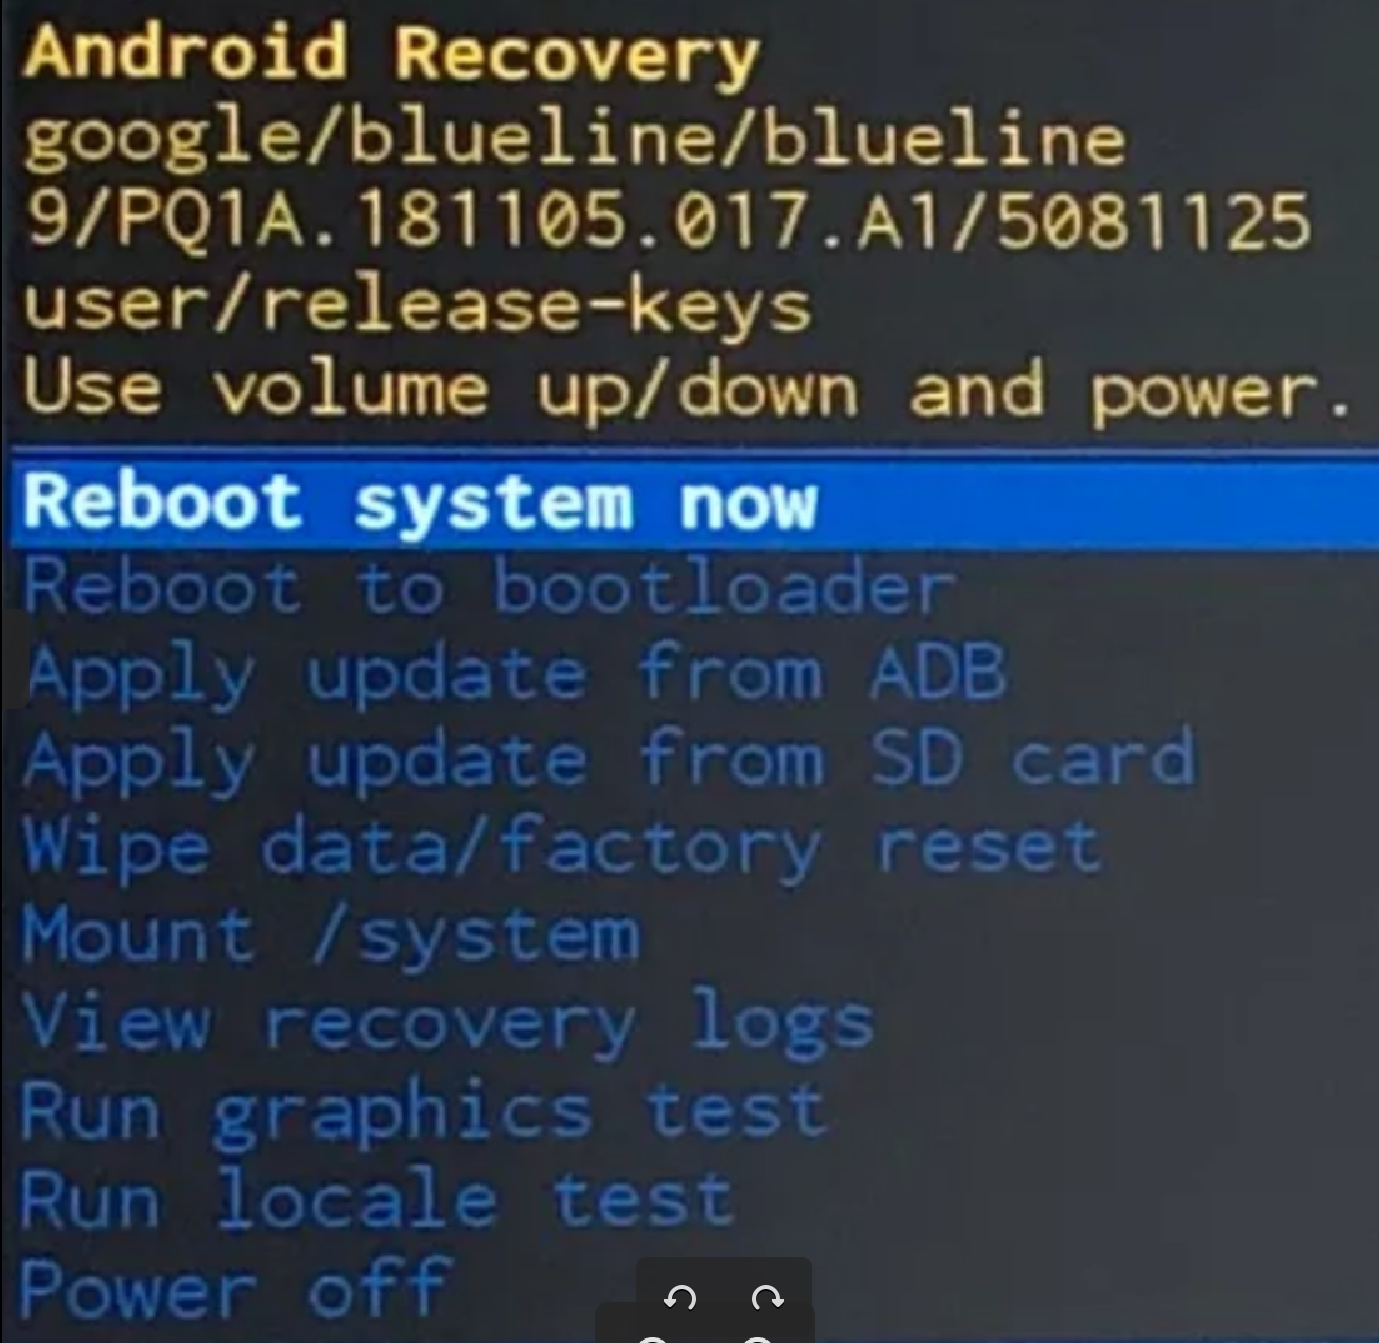
\includegraphics[width=0.5\columnwidth]{images/recovery.png}
    \caption{Foto da tela de recuperação de dados de um dispositivo Android.}
    \label{fig:recovery}
\end{figure}

\subsection{Sobrescrita de dados}

Utilizaremos uma distribuição Linux para todo o processo abaixo.

Para realizar a destruição de dados, primeiro precisamos explorar as partições do nosso dispositivo para identificar onde os dados que desejamos explorar estão armazenados. Para isso, temos algumas opções.

Primeiro, precisamos habilitar o "USB debugging" no dispositivo. Isso é feito em "Developer Options". Para habilitar as "Developer Options", precisamos clicar 7 vezes em "Build Number" em "About Phone".

Com o dispositivo conectado ao computador, podemos tentar acessar as partições diretamente com o comando "fdisk -l". Se o dispositivo permitir, para sobrescrever os dados, basta identificar a maior partição do dispositivo e utilizar uma ferramenta como o "shred" para sobrescrever todos os dados dela.

Possivelmente, o dispositivo não permitirá o acesso direto às partições. Nesse caso, podemos utilizar o "adb" para acessar o dispositivo. Para isso, precisamos instalar o "adb" no computador e, com o "adb" instalado, podemos acessar o dispositivo usando o comando "adb shell".

Através do "adb", podemos navegar pelas partições do dispositivo e identificar onde os dados que desejamos sobrescrever estão armazenados.

O "adb" também permite que utilizemos ferramentas do nosso sistema no dispositivo Android. Para isso, basta executar, por exemplo, o comando "adb shell "su -c 'dd if=/dev/block/mmcblk0'".

Com acesso às partições, podemos utilizar a ferramenta de nossa preferência para realizar a sobrescrita dos dados.

Outra alternativa é a ferramenta "jmptfs"; alguns dispositivos serão reconhecidos como um dispositivo "MTP" ao invés de um dispositivo de armazenamento externo. Nesse caso, podemos utilizar o comando "jmptfs ~/pasta\_de\_destino" para montar o dispositivo e acessar as partições.

\newpage

\section{Recuperação de dados}

Muito do processo é similar ao que foi abordado na destruição de dados. Nesta etapa, nosso objetivo é recuperar informações cruciais, e para isso, precisamos identificar as partições presentes no dispositivo e empregar ferramentas de recuperação de dados especializadas, como o renomado "foremost" e o versátil "photorec".

O primeiro passo consiste em realizar a cópia do conteúdo das partições para o nosso computador. Essa tarefa pode ser executada utilizando a ferramenta "dd" para transferir as partições relevantes para o sistema local.

Com as partições agora disponíveis em nosso computador, podemos utilizar as capacidades do "foremost" e do "photorec" para realizar uma busca minuciosa por dados perdidos ou excluídos. Essas ferramentas possuem algoritmos avançados de recuperação que podem varrer as partições copiadas em busca de arquivos e informações.

Entretanto, é importante notar que dispositivos mais recentes geralmente possuem criptografia de dados robusta, o que torna a recuperação de informações um desafio considerável. Nesses cenários, é possível explorar a opção de utilizar o "adb" para tentar acessar o dispositivo Android e, assim, tentar recuperar os dados protegidos pela criptografia. Vale ressaltar que essa abordagem pode ser mais complexa.

\section{Recuperação do dispositivo}

Após da destruição de dados, é importante destacar que é possível restaurar o funcionamento do dispositivo. Para realizar essa restauração, basta utilizar a ferramenta "adb" para instalar uma nova imagem do sistema no dispositivo. Geralmente, essa imagem está disponível para download no site oficial do fabricante do dispositivo.

No entanto, é importante notar que alguns fabricantes não disponibilizam essas imagens de sistema, o que pode tornar o processo de restauração do dispositivo mais complexo. Em tais situações, é viável recorrer a ferramentas alternativas, como o "fastboot", que permite a instalação de uma nova imagem do sistema diretamente no dispositivo.

Há também fabricantes, como a Samsung, que oferecem ferramentas específicas, como o "Odin", para facilitar o processo de restauração. O "Odin" possibilita ao usuário a instalação de uma nova imagem do sistema, incluindo a imagem de recuperação do sistema e o bootloader, tornando a restauração completa e abrangente.

Portanto, a restauração do dispositivo após a destruição de dados pode variar de acordo com o fabricante e a disponibilidade de ferramentas específicas, mas em geral, é um procedimento factível com as ferramentas adequadas.

\section{Conclusões}

Chegamos à conclusão de que o experimento foi conduzido com êxito, apresentando resultados que se aproximaram das expectativas inicialmente estabelecidas. A análise do circuito Darlington proporcionou uma compreensão mais aprofundada do comportamento dos transistores, bem como das análises necessárias para sua polarização e controle.

Foi possível realizar a montagem do projeto e empreender uma análise específica do componente preponderante no circuito, o capacitor $C_2$. Essa análise revelou a influência significativa de $C_2$ na frequência de corte do circuito, proporcionando uma visão mais apurada de sua contribuição para o desempenho global do sistema.

% \section{Apêndice}

Abaixo se encontra o código utilizado para a análise simbólica e numérica do circuito.

\begin{python}
    #from google.colab import drive
    #drive.mount('/content/drive')

    # Updating sympy to version 1.12 for faster inverse laplace transform
    # You need to restart the environment for the changes to take action
    # You need to run it before every session, or else the version will
    # be 1.11.1

    from google.colab import files

    %pip install -q --upgrade sympy

    import sympy
    sympy.__version__

    import matplotlib.pyplot as plt
    from sympy import *
    from IPython.core.interactiveshell import InteractiveShell

    # Allows multiple latex formatted lines
    InteractiveShell.ast_node_interactivity = 'all'

    # init_session prints the result in latex format, and has some useful presets,
    # more information at: https://docs.sympy.org/latest/modules/interactive.html
    init_session(quiet=True)
    # Allows the use of unicode characters
    init_printing(use_unicode=True)

\end{python}

\begin{python}
    import matplotlib.pyplot as plt
    from sympy import *

    # init_session prints the result in latex format, and has some useful presets,
    # more information at: https://docs.sympy.org/latest/modules/interactive.html
    init_session(quiet=True)
    # Allows the use of unicode characters
    init_printing(use_unicode=True)

    R0, R1, R2, R3, R4, R5, R6, R7, R8, R9, R10, R11, R12, R13 = \
    symbols('R0 R1 R2 R3 R4 R5 R6 R7 R8 R9 R10 R11 R12 R13')

    Va0, Va1, Va2, Va3, Va4, Va5, Va6, Va7, Va8, Va9, Va10 = \
    symbols('Va0 Va1 Va2 Va3 Va4 Va5 Va6 Va7 Va8 Va9 Va10')

    V0, V1, V2, V3, V4, V5, V6, V7, V8, V9, V10 = \
    symbols('V0 V1 V2 V3 V4 V5 V6 V7 V8 V9 V10')

    Vo0, Vo1, Vo2, Vo3, Vo4, Vo5, Vo6, Vo7, Vo8, Vo9, Vo10 = \
    symbols('Vo0 Vo1 Vo2 Vo3 Vo4 Vo5 Vo6 Vo7 Vo8 Vo9 Vo10')

    Vl0, Vl1, Vl2, Vl3, Vl4, Vl5, Vl6, Vl7, Vl8, Vl9, Vl10 = \
    symbols('Vl0 Vl1 Vl2 Vl3 Vl4 Vl5 Vl6 Vl7 Vl8 Vl9 Vl10')

    array_resistores = [R0, R1, R2, R3, R4, R5, R6, R7, R8, R9, R10, R11, R12, R13]

    Va = [Va0, Va1, Va2, Va3, Va4, Va5, Va6, Va7, Va8, Va9, Va10]

    V = [V0, V1, V2, V3, V4, V5, V6, V7, V8, V9, V10]

    Vo = [Vo0, Vo1, Vo2, Vo3, Vo4, Vo5, Vo6, Vo7, Vo8, Vo9, Vo10]

    Vl = [Vl0, Vl1, Vl2, Vl3, Vl4, Vl5, Vl6, Vl7, Vl8, Vl9, Vl10]

\end{python}

\begin{python}
    # Recebe um array de resistores e calcula a resistencia equivalente
    def paralelo(array_resistor, jump):
    sum = 0
    for i in range(len(array_resistor)):
    if i != jump:
    sum += 1/array_resistor[i]

    return 1/sum

    # Recebe um vetor de tensoes de entrada e um vetor de resistores ambos de mesmo tamanho e retorna o vetor com as tensoes de saida
    def divisorTensao(Vin, Vout ,resistores):
    for i in range(len(Vout)):
    Req = paralelo(resistores, i)
    Vout[i] = Vin[i]*Req/(resistores[i] + Req)
    return Vout
\end{python}

\begin{python}

    Va[0:4]=[0]*4
    Va[4:10] = divisorTensao(V[4:10], Va[4:10], array_resistores[4:10])
    Va[10] = 0
    Va

    for i in range(len(Vo)):
    if i<4:
    Vo[i]=0
    elif i<10:
    Vo[i] = Va[i]*(1 + array_resistores[11]/array_resistores[10])
    else:
    Vo[i] = -2.5*V[i]*array_resistores[11]/array_resistores[10]
    Vo

    for i in range(len(Vl)):
    if i<4:
    Vl[i] = -V[i]*array_resistores[13]/array_resistores[i]
    else:
    Vl[i] = -Vo[i]*(array_resistores[13]/array_resistores[12])
    Vl

    #K1 = R13
    #K2 = (R13/R12)(1+(R11/R10))
    #S10 = (2.5*R11*R13)/(R10*R12)

\end{python}

% \section{Anexos}

Código utilizado para geração de gráficos de bode, e análise utilizando as frequências de cortes obtidas experimentalmente.

\begin{python}
    import numpy as np
    import matplotlib.pyplot as plt
    from scipy.optimize import curve_fit



    fc1 = 210000
    fc2 = 11800


    freqs1 = np.array([0.002*fc1, 0.01*fc1, 0.05*fc1, 0.2*fc1, 0.5*fc1,
            0.8*fc1, fc1, 2*fc1, 4*fc1, 10*fc1, 20*fc1, 40*fc1])
    vin1 = np.array([0.2975, 0.297, 0.298, 0.297, 0.298,
            0.301, 0.297, 0.297, 0.3, 0.302, 0.301, 0.315])
    vout1 = np.array([1.404, 1.405, 1.403, 1.393, 1.306, 1.124,
            0.975, 0.54, 0.276, 0.114, 0.057, 0.031])


    freqs2 = np.array([0.05*fc2, 0.1*fc2, 0.2*fc2, 0.5*fc2, 0.8*fc2, fc2,
            2*fc2, 5*fc2, 20*fc2, 50*fc2, 200*fc2, 500*fc2, 1000*fc2])
    vin2 = np.array([0.1191, 0.1199, 0.12, 0.121, 0.122, 0.122,
            0.1218, 0.123, 0.123, 0.121, 0.121, 0.125, 0.151])
    vout2 = np.array([14.01, 13.95, 13.77, 12.61, 10.85, 9.8, 5.92,
            2.548, 0.645, 0.258, 0.0652, 0.0205, 0.0122])




    def mag_sqr_fun(f, K, fc):
    return (K*fc)**2/(f**2 + fc**2)


    def dB(m):
    return 20*np.log10(m)




    (K1, fc1), _ = curve_fit(lambda f, K, fc: dB(mag_sqr_fun(f, K, fc)),
    freqs1, 2*dB(vout1/vin1))


    print(f"""O ganho K eh {round(K1, 1)}
    A frequencia de corte eh {round(fc1, 1)} Hz""")

    f1 = np.logspace(np.log10(freqs1[0]) - 1, np.log10(freqs1[-1]) + 0.3)
    mag1 = dB(mag_sqr_fun(f1, K1, fc1))/2

    plt.semilogx(f1, mag1)
    plt.semilogx(freqs1, dB(vout1/vin1), "*")
    plt.xlabel("Freq (Hz)")
    plt.ylabel("Mag(H) (dB)")
    plt.title("Grafico de Bode de magnitude para o 1 circuito")
    plt.grid()
    plt.savefig("figura1.png")
    plt.show()



    (K2, fc2), _ = curve_fit(lambda f, K, fc: dB(mag_sqr_fun(f, K, fc)),
    freqs2, 2*dB(vout2/vin2))

    print("\n\nResultados para o 2 circuito:\n")
    print(f"""O ganho K eh {round(K2, 1)}
    A frequencia de corte eh {round(fc2, 1)} Hz""")

    f2 = np.logspace(np.log10(freqs2[0]) - 1, np.log10(freqs2[-1]) + 0.3)
    mag2 = dB(mag_sqr_fun(f2, K2, fc2))/2

    plt.semilogx(f2, mag2)
    plt.semilogx(freqs2, dB(vout2/vin2), "*")
    plt.xlabel("Freq (Hz)")
    plt.ylabel("Mag(H) (dB)")
    plt.title("Grafico de Bode de magnitude para o 2 circuito")
    plt.grid()
    plt.savefig("figura2.png")
    plt.show()




    plt.semilogx(f1, mag1)
    plt.semilogx(f2, mag2)
    plt.semilogx(freqs1, dB(vout1/vin1), "*")
    plt.semilogx(freqs2, dB(vout2/vin2), "*")
    plt.xlabel("Freq (Hz)")
    plt.ylabel("Mag(H) (dB)")
    plt.title("Grafico de Bode de magnitude para ambos os circuitos")
    plt.grid()
    plt.savefig("figura3.png")
    plt.show()

\end{python}


\end{document}